\documentclass[chi_draft]{sigchi}

% Use this command to override the default ACM copyright statement
% (e.g. for preprints).  Consult the conference website for the
% camera-ready copyright statement.

%% EXAMPLE BEGIN -- HOW TO OVERRIDE THE DEFAULT COPYRIGHT STRIP -- (July 22, 2013 - Paul Baumann)
% \toappear{Permission to make digital or hard copies of all or part of this work for personal or classroom use is      granted without fee provided that copies are not made or distributed for profit or commercial advantage and that copies bear this notice and the full citation on the first page. Copyrights for components of this work owned by others than ACM must be honored. Abstracting with credit is permitted. To copy otherwise, or republish, to post on servers or to redistribute to lists, requires prior specific permission and/or a fee. Request permissions from permissions@acm.org. \\
% {\emph{CHI'14}}, April 26--May 1, 2014, Toronto, Canada. \\
% Copyright \copyright~2014 ACM ISBN/14/04...\$15.00. \\
% DOI string from ACM form confirmation}
%% EXAMPLE END -- HOW TO OVERRIDE THE DEFAULT COPYRIGHT STRIP -- (July 22, 2013 - Paul Baumann)

% Arabic page numbers for submission.  Remove this line to eliminate
% page numbers for the camera ready copy
\pagenumbering{arabic}

\usepackage{times}
\usepackage{url}
\usepackage[pdftex]{hyperref}
\usepackage[T1]{fontenc}
\usepackage[utf8]{inputenc}
\usepackage[acronym]{glossaries}
\usepackage{blindtext, graphicx}
\usepackage{setspace}
% \usepackage{showframe}
\usepackage{enumitem}
\usepackage{tabularx, colortbl}
\usepackage[table]{xcolor}
\usepackage{array,ragged2e}
\usepackage{booktabs}
\usepackage{csquotes}
\usepackage[english]{babel}

\usepackage{balance}  % to better equalize the last page
\usepackage{txfonts}
\usepackage{mathptmx}
\usepackage{textcomp}
% Some optional stuff you might like/need.
\usepackage{microtype} % Improved Tracking and Kerning
% \usepackage[all]{hypcap}  % Fixes bug in hyperref caption linking
\usepackage{ccicons}  % Cite your images correctly!

% If you want to use todo notes, marginpars etc. during creation of your draft document, you
% have to enable the "chi_draft" option for the document class. To do this, change the very first
% line to: "\documentclass[chi_draft]{sigchi}". You can then place todo notes by using the "\todo{...}"
% command. Make sure to disable the draft option again before submitting your final document.
\usepackage{todonotes}

% Paper metadata (use plain text, for PDF inclusion and later
% re-using, if desired).  Use \emtpyauthor when submitting for review
% so you remain anonymous.
\def\plaintitle{COSC411 Assignment}
\def\plainauthor{Dion Woolley, Andy Cockburn}
\def\emptyauthor{}
\def\plainkeywords{rubberedge; pointing; clutching; elastic; isotonic; COSC411}
\def\plaingeneralterms{Pointing; Clutching}

% llt: Define a global style for URLs, rather that the default one
\makeatletter
\def\url@leostyle{%
  \@ifundefined{selectfont}{
    \def\UrlFont{\sf}
  }{
    \def\UrlFont{\small\bf\ttfamily}
  }}
\makeatother
\urlstyle{leo}

% To make various LaTeX processors do the right thing with page size.
\def\pprw{8.5in}
\def\pprh{11in}
\special{papersize=\pprw,\pprh}
\setlength{\paperwidth}{\pprw}
\setlength{\paperheight}{\pprh}
\setlength{\pdfpagewidth}{\pprw}
\setlength{\pdfpageheight}{\pprh}

% Make sure hyperref comes last of your loaded packages, to give it a
% fighting chance of not being over-written, since its job is to
% redefine many LaTeX commands.
\definecolor{linkColor}{RGB}{6,125,233}
\hypersetup{%
  pdftitle={\plaintitle},
% Use \plainauthor for final version.
%  pdfauthor={\plainauthor},
  pdfauthor={\emptyauthor},
  pdfkeywords={\plainkeywords},
  bookmarksnumbered,
  pdfstartview={FitH},
  colorlinks,
  citecolor=black,
  filecolor=black,
  linkcolor=black,
  urlcolor=linkColor,
  breaklinks=true,
}

% create a shortcut to typeset table headings
% \newcommand\tabhead[1]{\small\textbf{#1}}


\newacronym{CD}{CD}{Control-Display}
\newacronym{PPI}{PPI}{Pixels Per Inch}
\newacronym{API}{API}{Application Programming Interface}
\newacronym{ID}{ID}{Indices of Difficulty}
\makeglossaries

\graphicspath{ {images/} }


\begin{document}


% Hides copy right notice
\makeatletter
\def\@copyrightspace{\relax}
\makeatother


    \title{COSC411 Assignment}
\numberofauthors{2}
\author{
  \alignauthor Dion Woolley\\
    \affaddr{Department of Computer Science and\\Software Engineering}\\
    \affaddr{University of Canterbury}\\
    \email{dmw99@uclive.ac.nz}
  \alignauthor Andy Cockburn\\
    \affaddr{Department of Computer Science and\\Software Engineering}\\
    \affaddr{University of Canterbury}\\
    \email{andrew.cockburn@canterbury.ac.nz}
}

\maketitle

    \begin{abstract}
    This paper explores the use of a hybrid touchpad interaction technique through the use of a physical augmentation to existing touchpads, called RubberEdge. It aims to reduce clutches and the time take for a user to navigate between pointer targets when compared to conventional touchpad transfer functions, specifically Constant Gain and Acceleration. We found that our implementation of RubberEdge was successful at reducing the number of clutch movements when compared to Constant or Acceleration functions by (14\% - 42\%), depending on the distance of the movement. However, there were no significant results found for selection time of targets. The data suggests that the current implementation of the RubberEdge transfer function is worse than existing Constant and Acceleration functions. This is due to flaws in the experiment implementation, with time permitting would have been resolved before the experiment was conducted.
\end{abstract}

% \category{H.5.m.}{Information Interfaces and Presentation
%   (e.g. HCI)}{Miscellaneous} \category{See
%   \url{http://acm.org/about/class/1998/} for the full list of ACM
%   classifiers. This section is required.}{}{}

\keywords{\plainkeywords}

    \section{Introduction}
Clutching occurs when a users required more than one finger action to perform a pointer movement. In a classic example of this a user wishes to move the pointer from one end of the screen to the other but runs out of room on their touchpad to complete the movement in a single action, so they are required to reset their finger position a number of times to complete the movement. Because multiple movements are required time is wasted between each clutch invocation, compared to if the pointer movement could be achieved in one motion.

    \section{Background and Related Work}

This work is based on the initial work done in the RubberEdge paper\cite{Casiez2007RubberEdge}, where this paper is evaluating a more advanced version of their prototype design for RubberEdge. Conditions have changed in touchpads and screen interaction since the paper was published. Specifically the introduction of high-resolution 4k displays and display scaling as well as newer pointer acceleration curves and larger touch pads.

From the perspective of a touchpad user, we still using clutching in our everyday interactions. So despite the growing size of trackpads clutching still occurs. Whether or not clutching is bad is debatable \cite{Nancel2015ClutchingEnemy} argues that pointer movements are possible without clutching but is detrimental for target selection time and induces more errors. So some clutching is beneficial, and it is not solely caused by a lack of touchpad space.

Over the years touch pads have increased in their overall size, this is likely due to the increasing availability of gestures. However, it is noted that there is no significant improvement in the usability for pointing tasks when using a larger touchpad over a smaller one\cite{Avera2016EffectsPerformance}. The size of the touchpad may impact the type of gestures that can be used.

The density of screens has increased, with it now being common to see laptops with resolutions of 4k (3840 x 2160) or greater on the market. There is also a larger variety of screen aspect ratios, with 16:9 remaining dominate, also significant is 16:10 on MacBooks\cite{MacBookProNZ} and 3:2 on Microsoft's Surface\cite{SurfaceBeauty} line of products having a significant share of the market. However, the increased resolution is offset by the use of display scaling; this means the effective resolution is a lot lower than the native resolution, often it is between 1080p and 1440p.

The current methods for user input are; fixed ratio of display movement to control movement \gls{CD} (a scaling factor, 1mm movement on the touchpad equates to x number of pixels moved in the same direction). The alternative is pointer cursor acceleration, which depends on the velocity of the input on the touchpad. A low velocity equates to a low \gls{CD} gain this improves pointer precision and a high \gls{CD} gain at high velocity, to cover a large distance while minimise clutching.

For hybrid position and rate control techniques, it was found that without haptic feedback transitioning between position and rate mode was difficult to distinguish. However, elastic feedback is well suited to rate control.

Three types of input devices, isotonic, isometric and elastic. Isotonic free moving uses position input (mouse, touchpad). Isometric devices (TrackPoint)\cite{ZhaiHumanControl} do not move and use force for input. In between these two device types are elastic devices, which use a mix of force and position for input.

RubberEdge is a hybrid between isotonic and isometric, where there is an isotonic zone for precise input, and an isometric or elastic zone, for use when faster pointer movement is required, which provides force feedback relative to the acceleration of the pointer.

    \section{RubberEdge Device}

\begin{figure}[h]
    \centering
    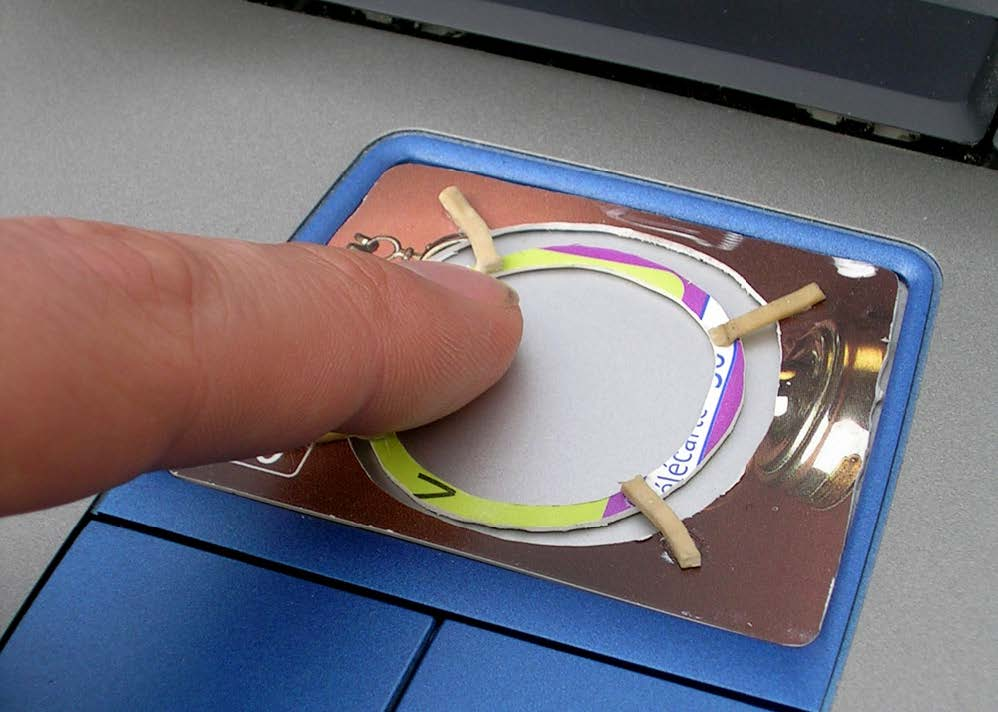
\includegraphics[width=0.9\columnwidth]{Existing}
    \caption{The RubberEdge interface from the previous study on RubberEdge \protect\cite{Casiez2007RubberEdge}}
    \label{fig:existing}
\end{figure}

This research paper aims to improve upon an existing RubberEdge implementation. The paper\cite{Casiez2007RubberEdge} that this research draws inspiration from only empirically examines their implementation of the RubberEdge as shown in Figure \ref{fig:existing}. The experimental results show in the paper were gathered with a Phantom Omni haptic device\cite{GeomagicOverview}, this apparatus mocked the feeling of RubberEdge to the participant. Although the interaction was not quite the same as it would be with a real touchpad, as the participant would not get the same feedback from physically pushing up against a ring over feeling some resistance. This research started with creating a RubberEdge apparatus using the existing design from the source paper.

\subsection{Interface Design}
The initial design called for a device which would sit neatly over a touchpad on a laptop. Measurements of the laptop's touchpad were 105mm x 80mm, after accounting for structural integrity of the edges of the interface, the design left a circular area with a 30mm radius, for the isotonic zone and around 7.5mm of radius for the elastic zone, the actual available area is less due to the collapsing spring arms of the final design. This left a usable isotonic area of 2827mm$^2$

In the first iteration of the design, an initial attempt at replicating the existing design was attempted by laser cutting an outer frame and inner ring out of acrylic. This design was abandoned in favour of a solution suggested by the mechanical technician that helped with the laser cutting and subsequent 3D printing. They suggested that a solution using spring arms might be an effective alternative, a design was quickly drafted, and cut from acrylic. The design showed promise but unfortunately, the acrylic material proved to be too rigid, and the spring arms would break under force.

\begin{figure}[h]
    \centering
    
\includegraphics[width=0.9\columnwidth]{CADdesignV1}
    \caption{First design for the composite 3D printed RubberEdge interface.}
    \label{fig:cadv1}
\end{figure}

An alternative method of creating the interface was to use a composite 3D printer; this printer can blend multiple polymers to change the ply-ability of the plastic. A hybrid design was used where the outer frame and inner ring was printed with a rigid material, and the spring arms printed with an elastic type polymer, this design can be seen in Figure \ref{fig:cadv1}. The proprieties of the elastic material used are not freely available as the technology is proprietary to the manufacturer of the 3D printer, and material. The material is simply described as Shore 85, which only indicates the hardness of the material. Further tests should be conducted to evaluate the elasticity of the material to see if it falls in line with design guidelines present in this study\cite{Casiez2008TheDevice}.

\begin{figure}[h]
    \centering
    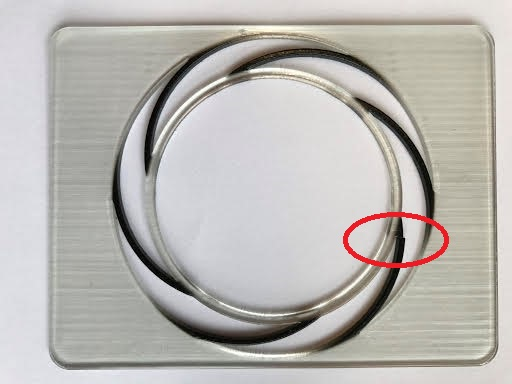
\includegraphics[width=0.9\columnwidth]{3Dprintv1}
    \caption{As shown in the red circle, a major problem of the first spring arm design was the spring arms breaking after a period of use.}
    \label{fig:3dprintv1}
\end{figure}

\begin{figure}[h]
    \centering
    
\includegraphics[width=0.9\columnwidth]{CADdesignV2}
    \caption{The final design of the RubberEdge interface used in the experiment.}
    \label{fig:cadv2}
\end{figure}

Problems occurred with the initial 3D printed design, the key of which was the spring arms breaking after a period of use. The arms broke due to them being stretched too far when the inner ring was pushed up against the wall of the outer frame. The next and final iteration of the design solved this problem by changing the spring arm design to allow the arms to extend and contract, as well as increasing the thickness of the spring arms from 1.5mm to 2mm; the final design can be seen in Figure \ref{fig:cadv2}.



\subsection{Interface Data}\label{section:interface_data}
Initially, in order to read the input from a participant using the RubberEdge device on the touchpad of a laptop the libpointing library\cite{Roussel2017Libpointing}\cite{Casiez2011NoFunctions} was used. However, after an investigation into the source code and the underlying Window's \glspl{API}\cite{RawWindows} there was no way to get the absolute position of a participants finger on the touchpad using libpointing. This is despite a method called getPosition() as part of the libpointing \gls{API}.

The authors of the reference paper used a touchpad driven by Synaptic's drivers, which could be installed on the laptop. At the time, Synaptic offered an SDK to interact with their drivers, however, it appears this is no longer offered on their website, and clones available on Github have not been kept up to date with the latest drivers.

The existing drivers on the laptop are for Windows precision touchpads. This driver provides two interfaces that a developer can subscribe to\cite{PrecisionGuide}. The first interface provides relative pointer events and is the one used by the libpointing library. The second interface positions itself as a generic touchscreen\cite{WindowsWindows}, this is used for gesture recognition and does provide the absolute coordinates for interactions with the touchpad.

Due to time constraints we were not able to use the newer driver interface, and instead found a compromise to the method of input as seen in Section \ref{section:apparatus}


    
    \section{Experiment}

\subsection{Goals and Hypothesis}
\textbf{H1}: RubberEdge will reduce clutch invocations required to traverse a pointer to a target when compared to conventional Transfer Functions, Constant Gain and Acceleration.

\textbf{H2}: The time taken to traverse a pointer to a target using the RubberEdge Function will be less than existing Constant and Acceleration Transfer Functions.


\subsection{Apparatus}\label{section:apparatus}
The laptop used for the experiments was a Dell XPS 15 9560\cite{XPSZealand}, it featured a 15 inch display with a resolution of 3840px x 2160px, giving it 282.4 \gls{PPI}. The Windows 10 operating system, with display scaling set to 175\% for an effective resolution of 2194px x 1234px was used on the laptop.

\begin{figure}[h]
    \centering
    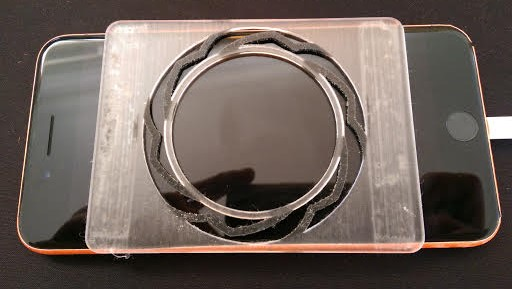
\includegraphics[width=0.9\columnwidth]{Aparatus}
    \caption{The RubberEdge device, adhered to the screen of an iPhone 7 Plus}
    \label{fig:apparatus}
\end{figure}

As discussed in Section \ref{section:interface_data} problems were encountered when getting the absolute position of a participants finger on the touchpad, due to time constraints a compromised was settled on where an iPhone 7 Plus was used, with the RubberEdge interface adhered to the screen with double sided tape, as shown in Figure \ref{fig:apparatus}. A separate web page was then created, that would be navigated to on the phone, from which touch input could be transmitted to the laptop hosting a web server over web sockets.


\subsection{Experiment Interface}
An experiment based on Fitts' law was deemed to be an adequate way of testing the conditions. The interface is based off the Visualising Fitts Law\cite{Wallner2017AnD3} web page, which follows the ISO 9241-9 standard\cite{ISODevices}

The web interface used in the experiment was built using the Polymer framework\cite{WelcomeProject}.

Participants were first presented with an instructions page outlining how the RubberEdge device is intended to be used. After completing a short pre-experiment survey, they calibrate the isotonic and elastic zones for their finger.
The calibration processed involved tracing with one finger around the edge of the inner ring of the RubberEdge device, without putting pressure on the ring. Calibration is important as participants had different sized fingers and would orient their hands differently relative to the device.

To calculate the isotonic and elastic zone a circle fitting algorithm\cite{Maisonobe2007FindingPoints} was applied which takes a set of points and finds the midpoint and radius of a circle that best represents those points. This circle defines the isotonic zone, points falling outside the circle are considered to be in the elastic zone.

From this entries in and out of the elastic zone can be tracked by measuring the distance between a given point and the centre of the defined isotonic zone.

\subsection{Task and Stimuli}
The Fitts' law task is to move the pointer in the indicated circle, upon which release the finger from the touchpad a new target would be generated. Nine targets are spaced equally around a central point, which is in the centre of the screen. Targets are selected in an opposing order, which means the user has to move the pointer and equal distance to select each target.

The distances selected based on relative pixel coordinates in the web browser were 500px, 750px, 1000px when translated to mm this works out to be 79mm, 118mm, 157mm respectively.
The selected widths were 25px, 50px, 75px and translated they are 3.9mm, 7.9mm, 11.8mm respectively.

\begin{figure}[h]
    \centering
    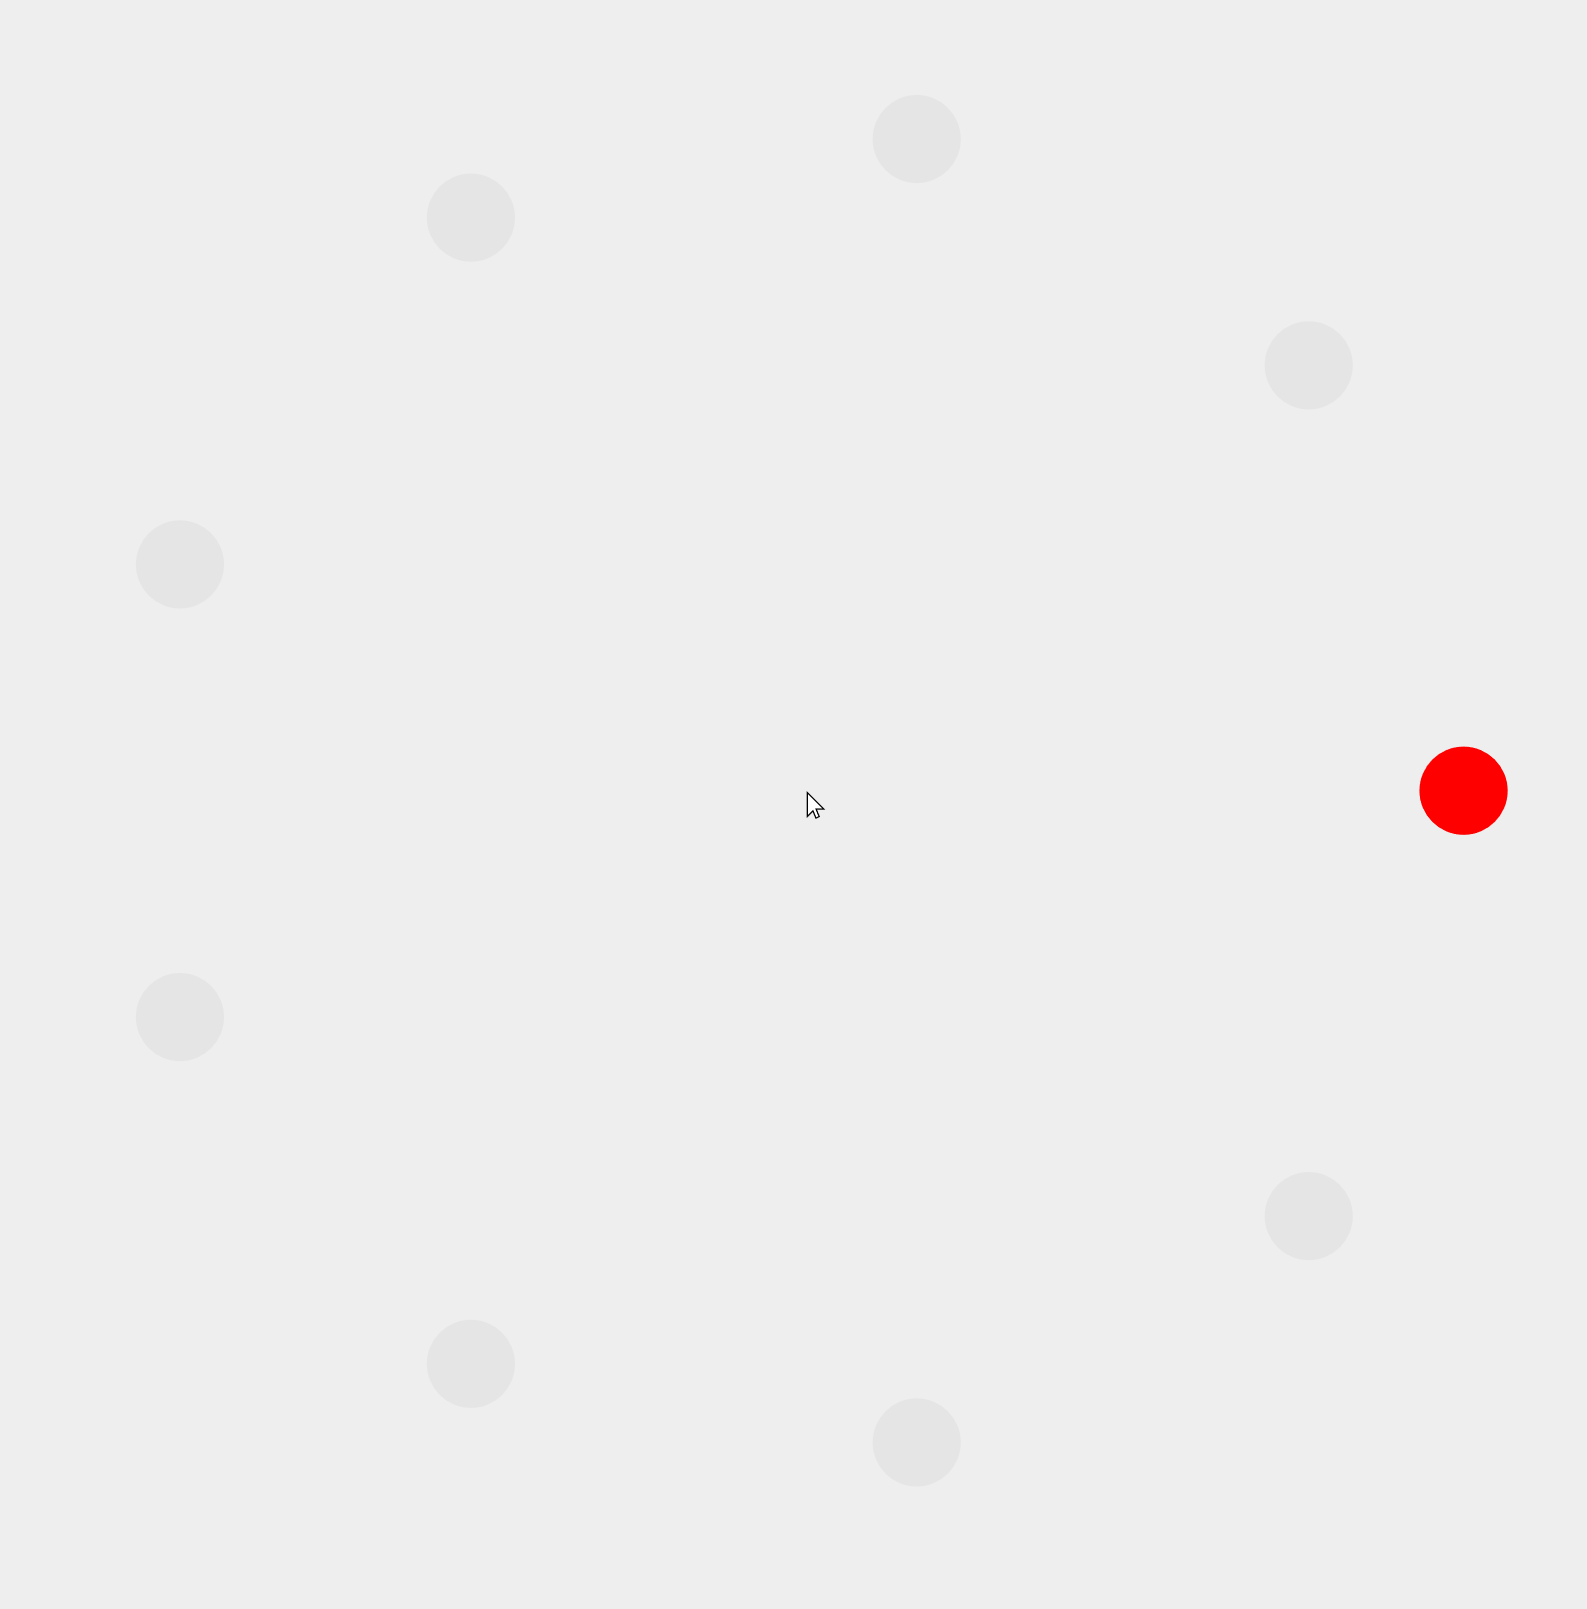
\includegraphics[width=0.9\columnwidth]{Interface}
    \caption{The Fitts' Law interface used by participants, with the target highlighted in red and possible targets in dark gray.}
    \label{fig:interface}
\end{figure}

After completing the calibration phase, participants are trained on each function, {Constant, Acceleration, RubberEdge} with a fixed distance (118mm) and width (7.9mm) of the targets, an example of the interface presented to participants is seen in Figure \ref{fig:interface}

Once training is complete, participants are presented with one of the three transfer functions and are asked to complete the task for all distance and width combinations. After which the combinations are repeated for the other transfer functions, with a 30 second break between each transfer function. The order of the distance and width combinations are randomised for each transfer function and each participant, using the Durstenfeld shuffle algorithm.

After completing the experiment, participants are asked to complete a survey evaluating each transfer function.

\subsection{Interface problems}\label{section:interface_problems}
A major flaw of the experiment was the transmission of data between the laptop and phone. Due to the instability of wireless communications, the pointer would move in a slightly staggered motion, often inducing a noticeable lag, this did affect the observed performance of the participants in the study. A solution to this problem would be changing the communication method to be over USB; however, the development time involved made this solution unfeasible.

\subsection{Participants}
Seven people (3 female, 4 male) participated in the experiment; participants were in the age range of (15 - 25) years, except for one in the age range of (45 - 55) years. Participants were asked the average number of hours spent using a touchpad each day; responses were varied from not using a touchpad at all to greater than 8 hours per day. Operating system use varied between participants, with five using Windows and one for each MacOS and Linux. Preference for existing pointer acceleration on touchpads also varied, four participants, preferred acceleration, one did not, and two either had no preference or did not know what pointer acceleration was.

\subsection{Design}
A within-subjects design was used. The independent variables were Transfer Function (Constant, Acceleration, RubberEdge), target Distance (D$_S$ - 79mm, D$_M$ 118mm, D$_L$ - 157mm) and target Widths (W$_S$ - 11.8mm, W$_M$ - 7.9mm, W$_S$ 3.9mm) The dependent variables measured were the time between selecting targets and the number of clutches performed to select a target.

Each distance and width combination is pre-set with a sequence of nine targets for the user to select. With three different distances and three widths makes nine unique distance and width combinations. This gave seven Fitts' \gls{ID}\cite{MacKenzie1992FittsInteraction}

For the Constant transfer function, a \gls{CD} gain of 2 was used, this was to encourage clutching and was similar to the default system transfer function provided by Windows 10. The acceleration transfer function was the default provided by Windows 10. The transfer function for RubberEdge in the isotonic was set to a \gls{CD} gain of 2. In the elastic zone, the average velocity of the last three data points from the isotonic zone is used as the initial velocity, from then an acceleration multiplier relative to the distance away from the edge of the isotonic and elastic zone is applied. When the participant is stationary in the elastic zone the pointer is updated at a rate of 400Hz, which is equivalent to the update rate of the touchpad of the laptop. A limit is applied on the maximum velocity that can be obtained by the pointer; this is to prevent the pointer running away from the participant and make the behaviour more predictable.

The order of the transfer functions was counterbalanced between participants using the Latin Squares method. This is to avoid any asymmetric skill transfer induced by training. 

The experiment lasted approximately 15 minutes.

The total number of trials conducted are:\\
7 Participants $\times$ 3 Transfer Functions $\times$ 3 Distances $\times$ 3 Widths $\times$ 9 targets\\
$=$ 1701 total trials

    \section{Results}
The dependent variables were selection time and the number of clutches.

\subsection{Selection Time}
Selection time is the time between each subsequent target selection. This means that the first target the participants selects for each Transfer Function is not included in the results. Outliers for trials over 20 seconds were removed from the data.

\begin{figure}[h]
    \centering
    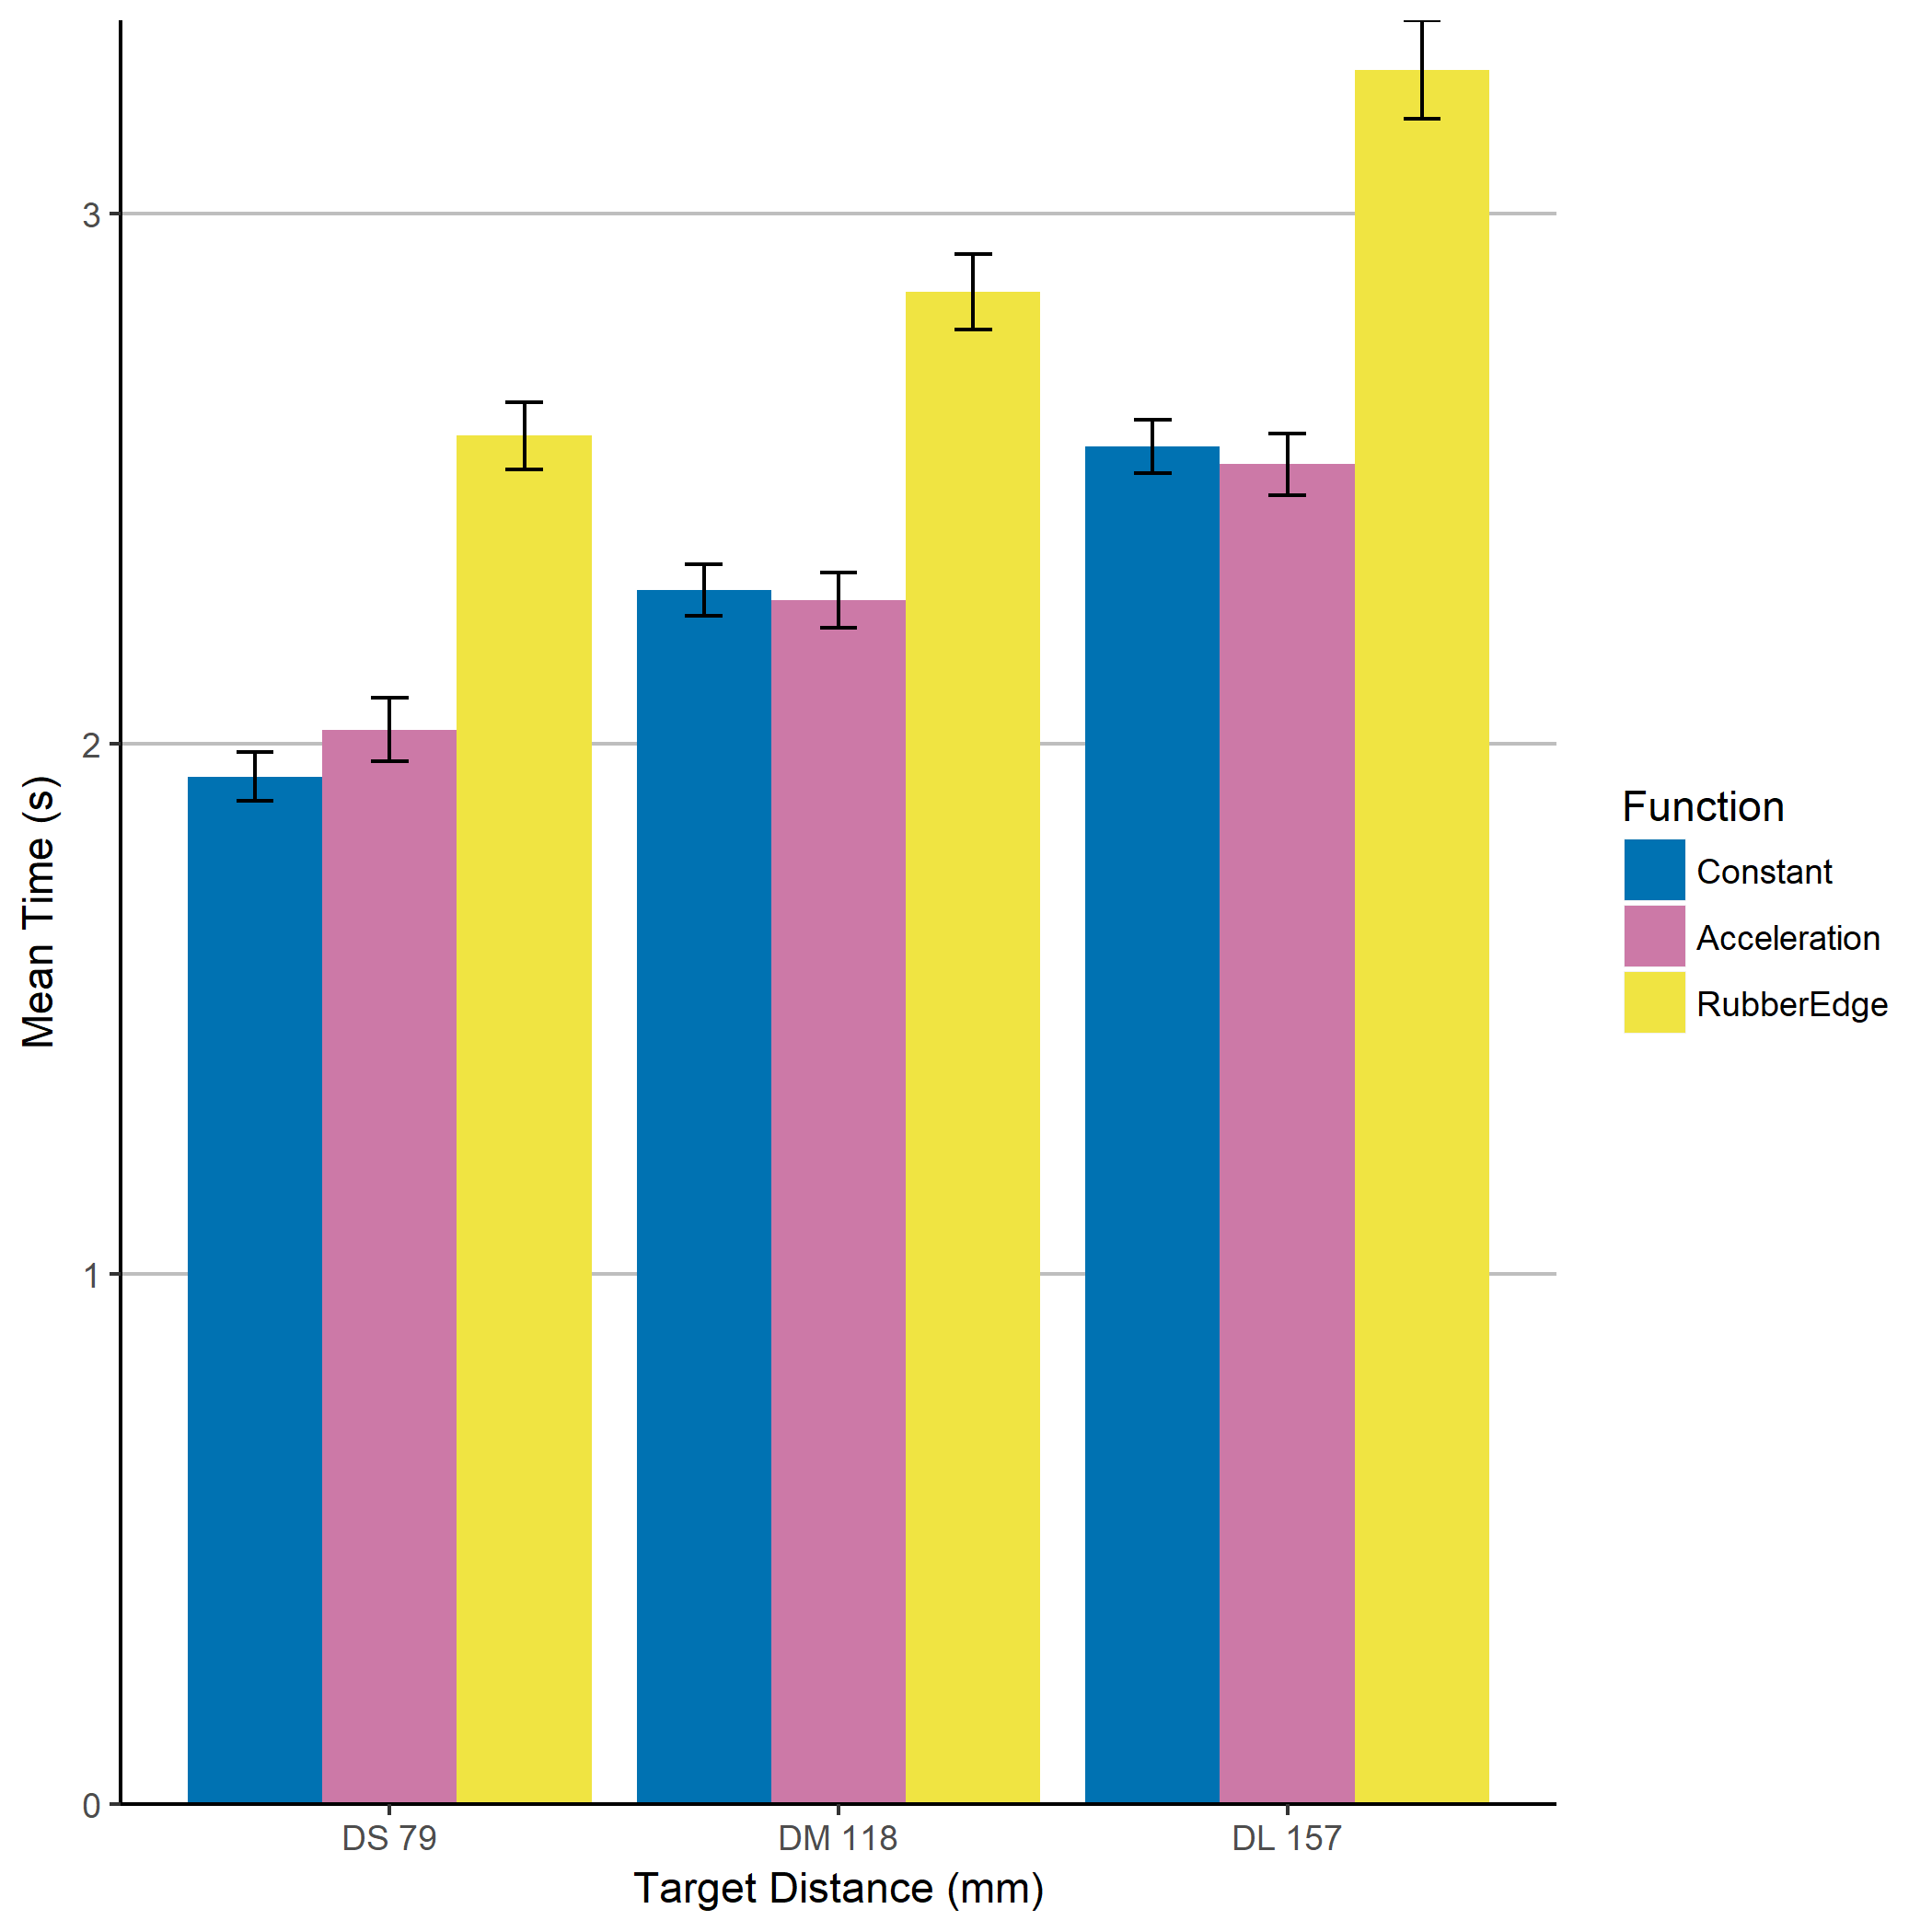
\includegraphics[width=0.9\columnwidth]{selection-time}
    \caption{Selection Time, Transfer Function x Distance Interaction}
    \label{fig:selection-time}
\end{figure}

Repeated measures analysis of variance using Mauchly's Test for Sphericity, showed that the order of Transfer Functions presented to the participant had no significant effect on movement time, so there was no significant asymmetric skill transfer, this indicated that the within-subjects design was appropriate. There was a significant main effect for the for the Transfer Function on selection time (F$_{2,12}$ = 10.3, p < 0.005) with the Constant and Acceleration outperforming the RubberEdge Transfer Function by 21.8\%, this can be seen across all distances in Figure \ref{fig:selection-time}. There was also a significant main effect for Distance (F$_{2,12}$ = 30.8, p < 0.0001) on selection time. The interaction between Transfer Function x Distance was not significant (F$_{2,24}$ = 0.70, p = 0.59). Therefore we cannot accept \textbf{H2}.

Pair-wise comparisons using Bonferroni found that there was a significant difference between RubberEdge and the Constant and Acceleration Transfer Functions. Another pair-wise test also found a significant difference between each distance (D$_S$, D$_M$, D$_L$)

\subsection{Fitts' Law Analysis}

\begin{figure}[h]
    \centering
    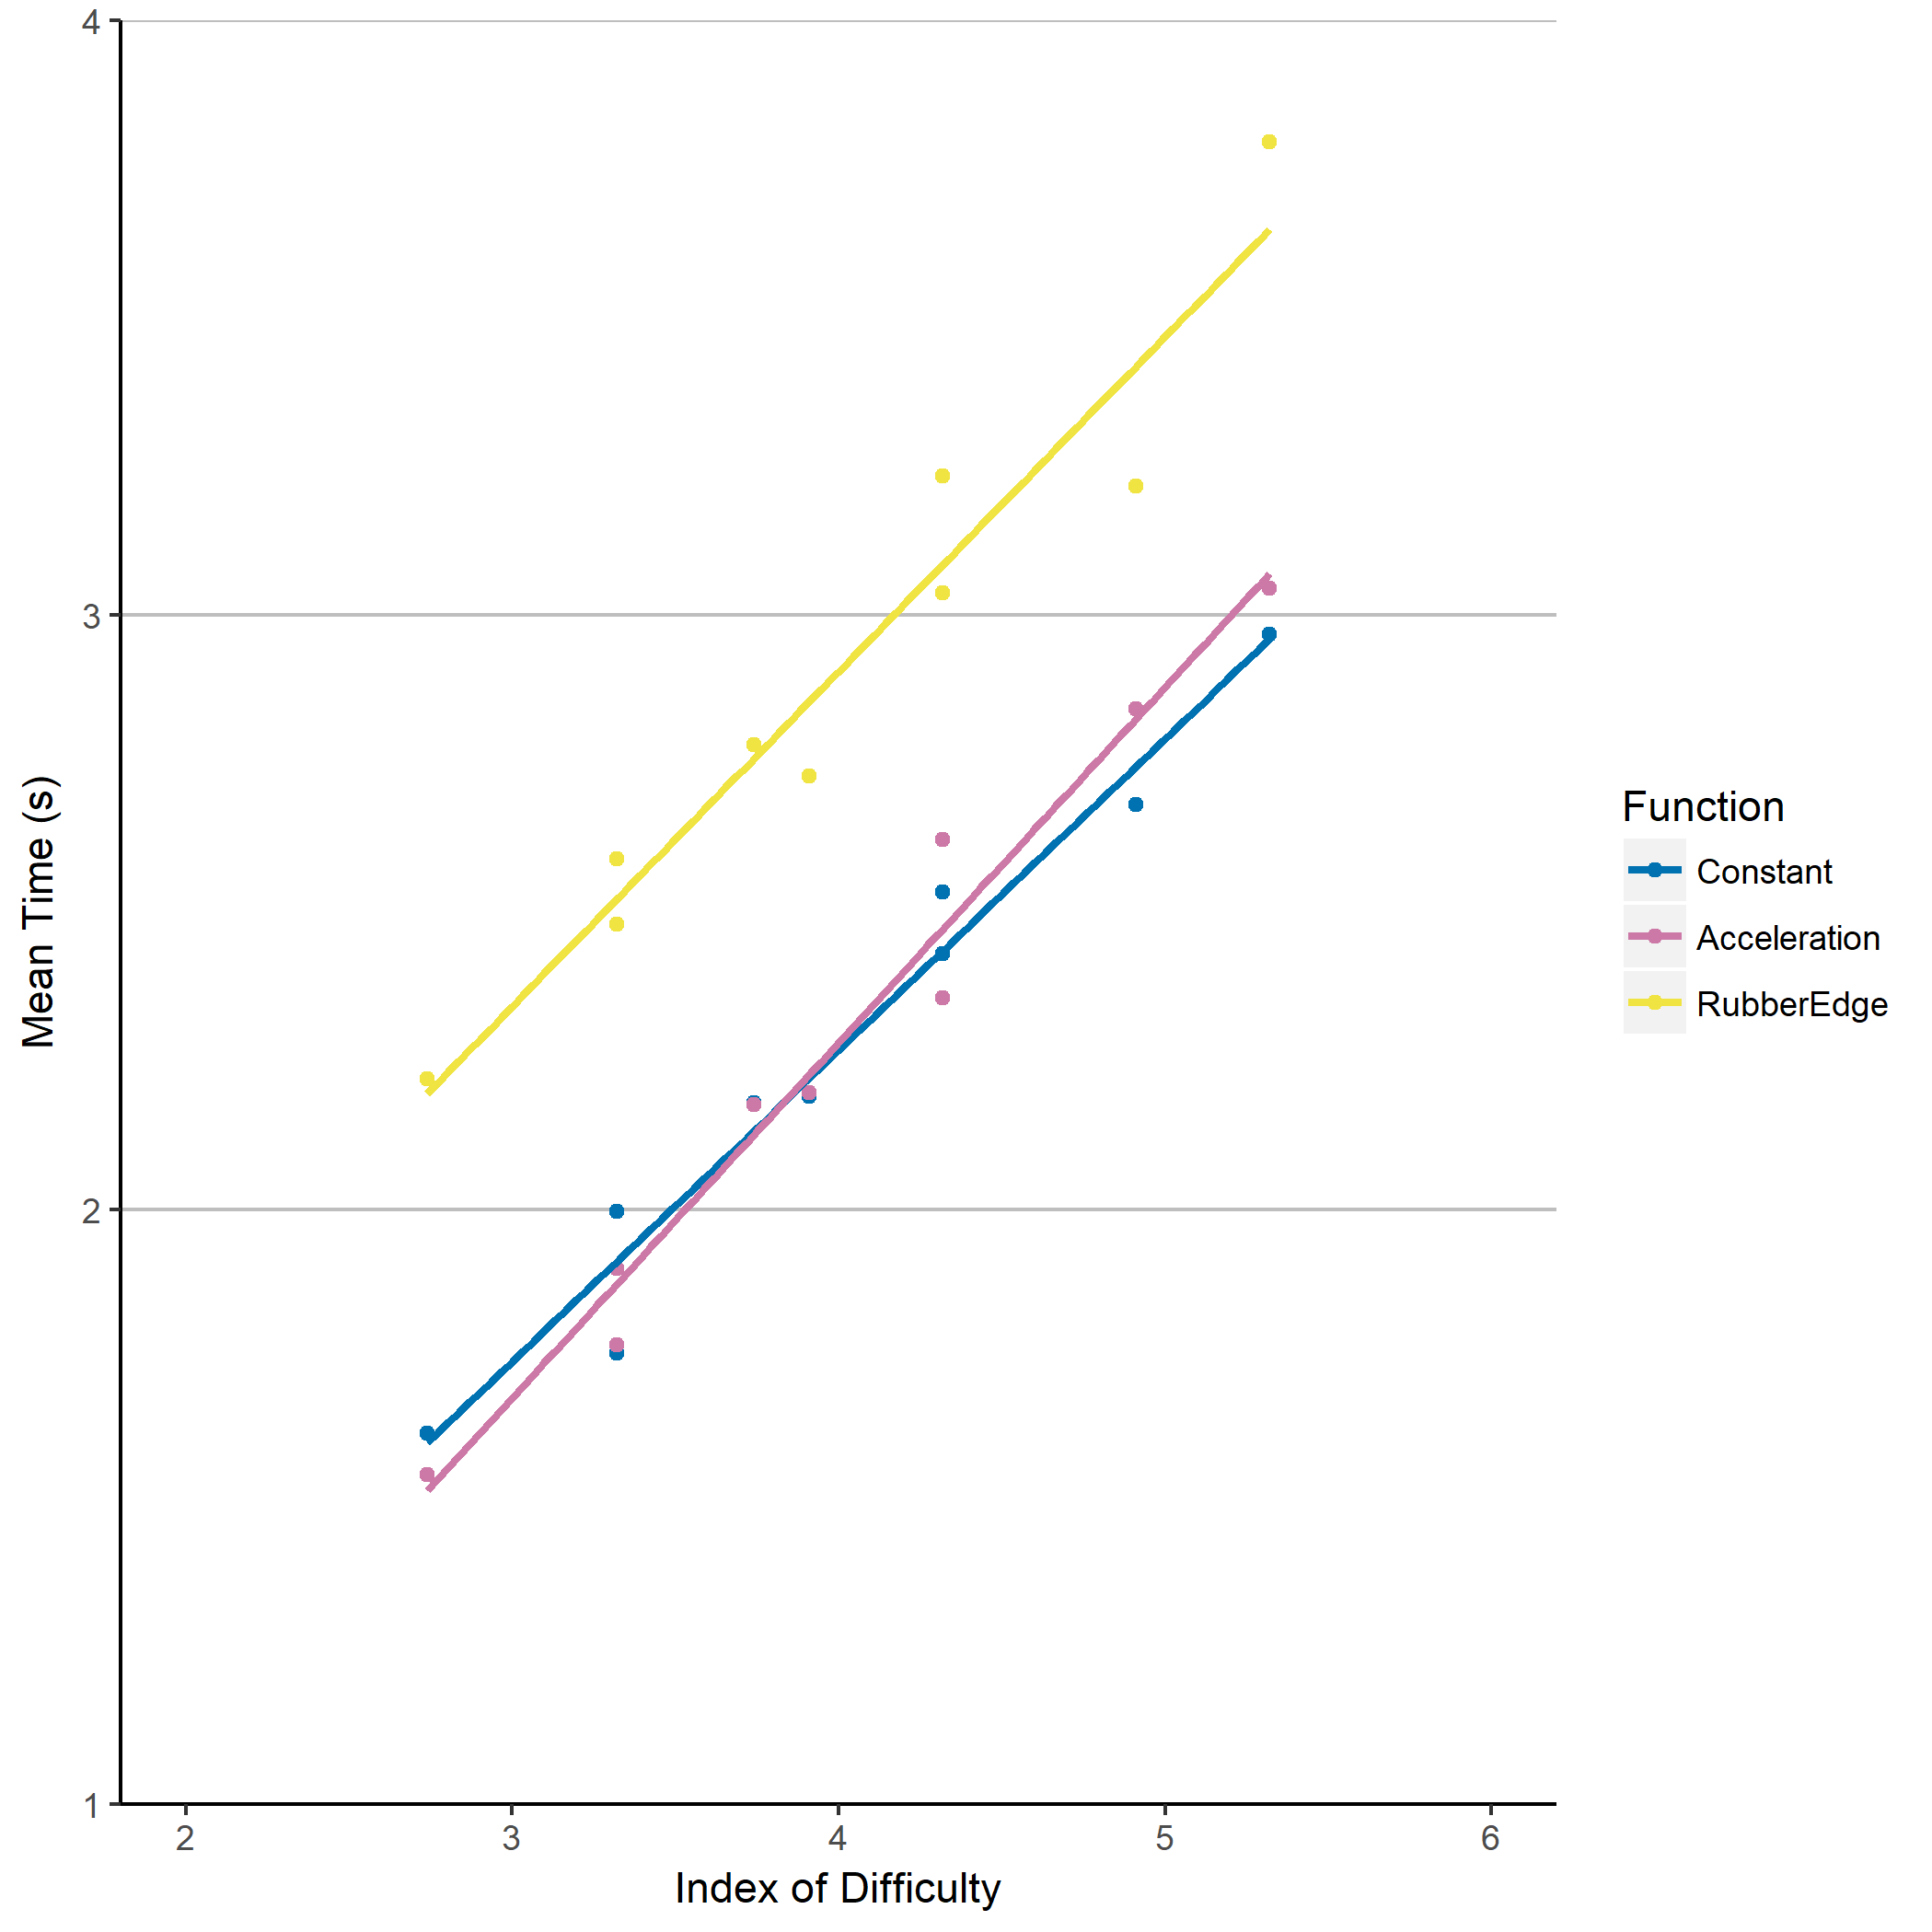
\includegraphics[width=0.9\columnwidth]{fitts}
    \caption{A comparison between the Index of difficulty and mean time, between different transfer functions.}
    \label{fig:fitts}
\end{figure}

A significant difference for Fitts' law between distances was not found (Figure \ref{fig:fitts}). Whereas the previous study\cite{Casiez2007RubberEdge} found that the distance had a significant effect for indexes of the same difficulty. Why the results found in this study differ, is likely because the distances measured against in the previous study were much larger, 172, 344, 688mm. Compared to 79, 118, 157mm for this study. The reason that smaller distances were chosen is that they align closer to distances that users are likely to demonstrate on a laptop device. Specifically, 157mm was around the limit for the distance from the centre point of the laptop screen to the upper or lower edge, see section \ref{section:apparatus} for details about the laptop used. 

\begin{table}[h]
\centering
{\rowcolors{2}{gray!30}{lightgray!30}
\begin{tabular}{ l r r r } 
 Function & $a$ & $b$ & $r^2$ \\ 
 \hline
 Constant & 0.20 & 0.52 & 0.99 \\ 
 Acceleration & -0.08 & 0.59 & 0.99 \\ 
 RubberEdge & 0.64 & 0.56 & 0.95 \\
 \hline
 \end{tabular}
}
\vspace{0.5cm}
 \caption{Fitts' Law regression values for different transfer functions, where $a$ is the intercept of the regression line, $b$ is the slope, $r^2$ is the fitness.}
\label{table:fitts}
\end{table}

\begin{figure}[h]
    \centering
    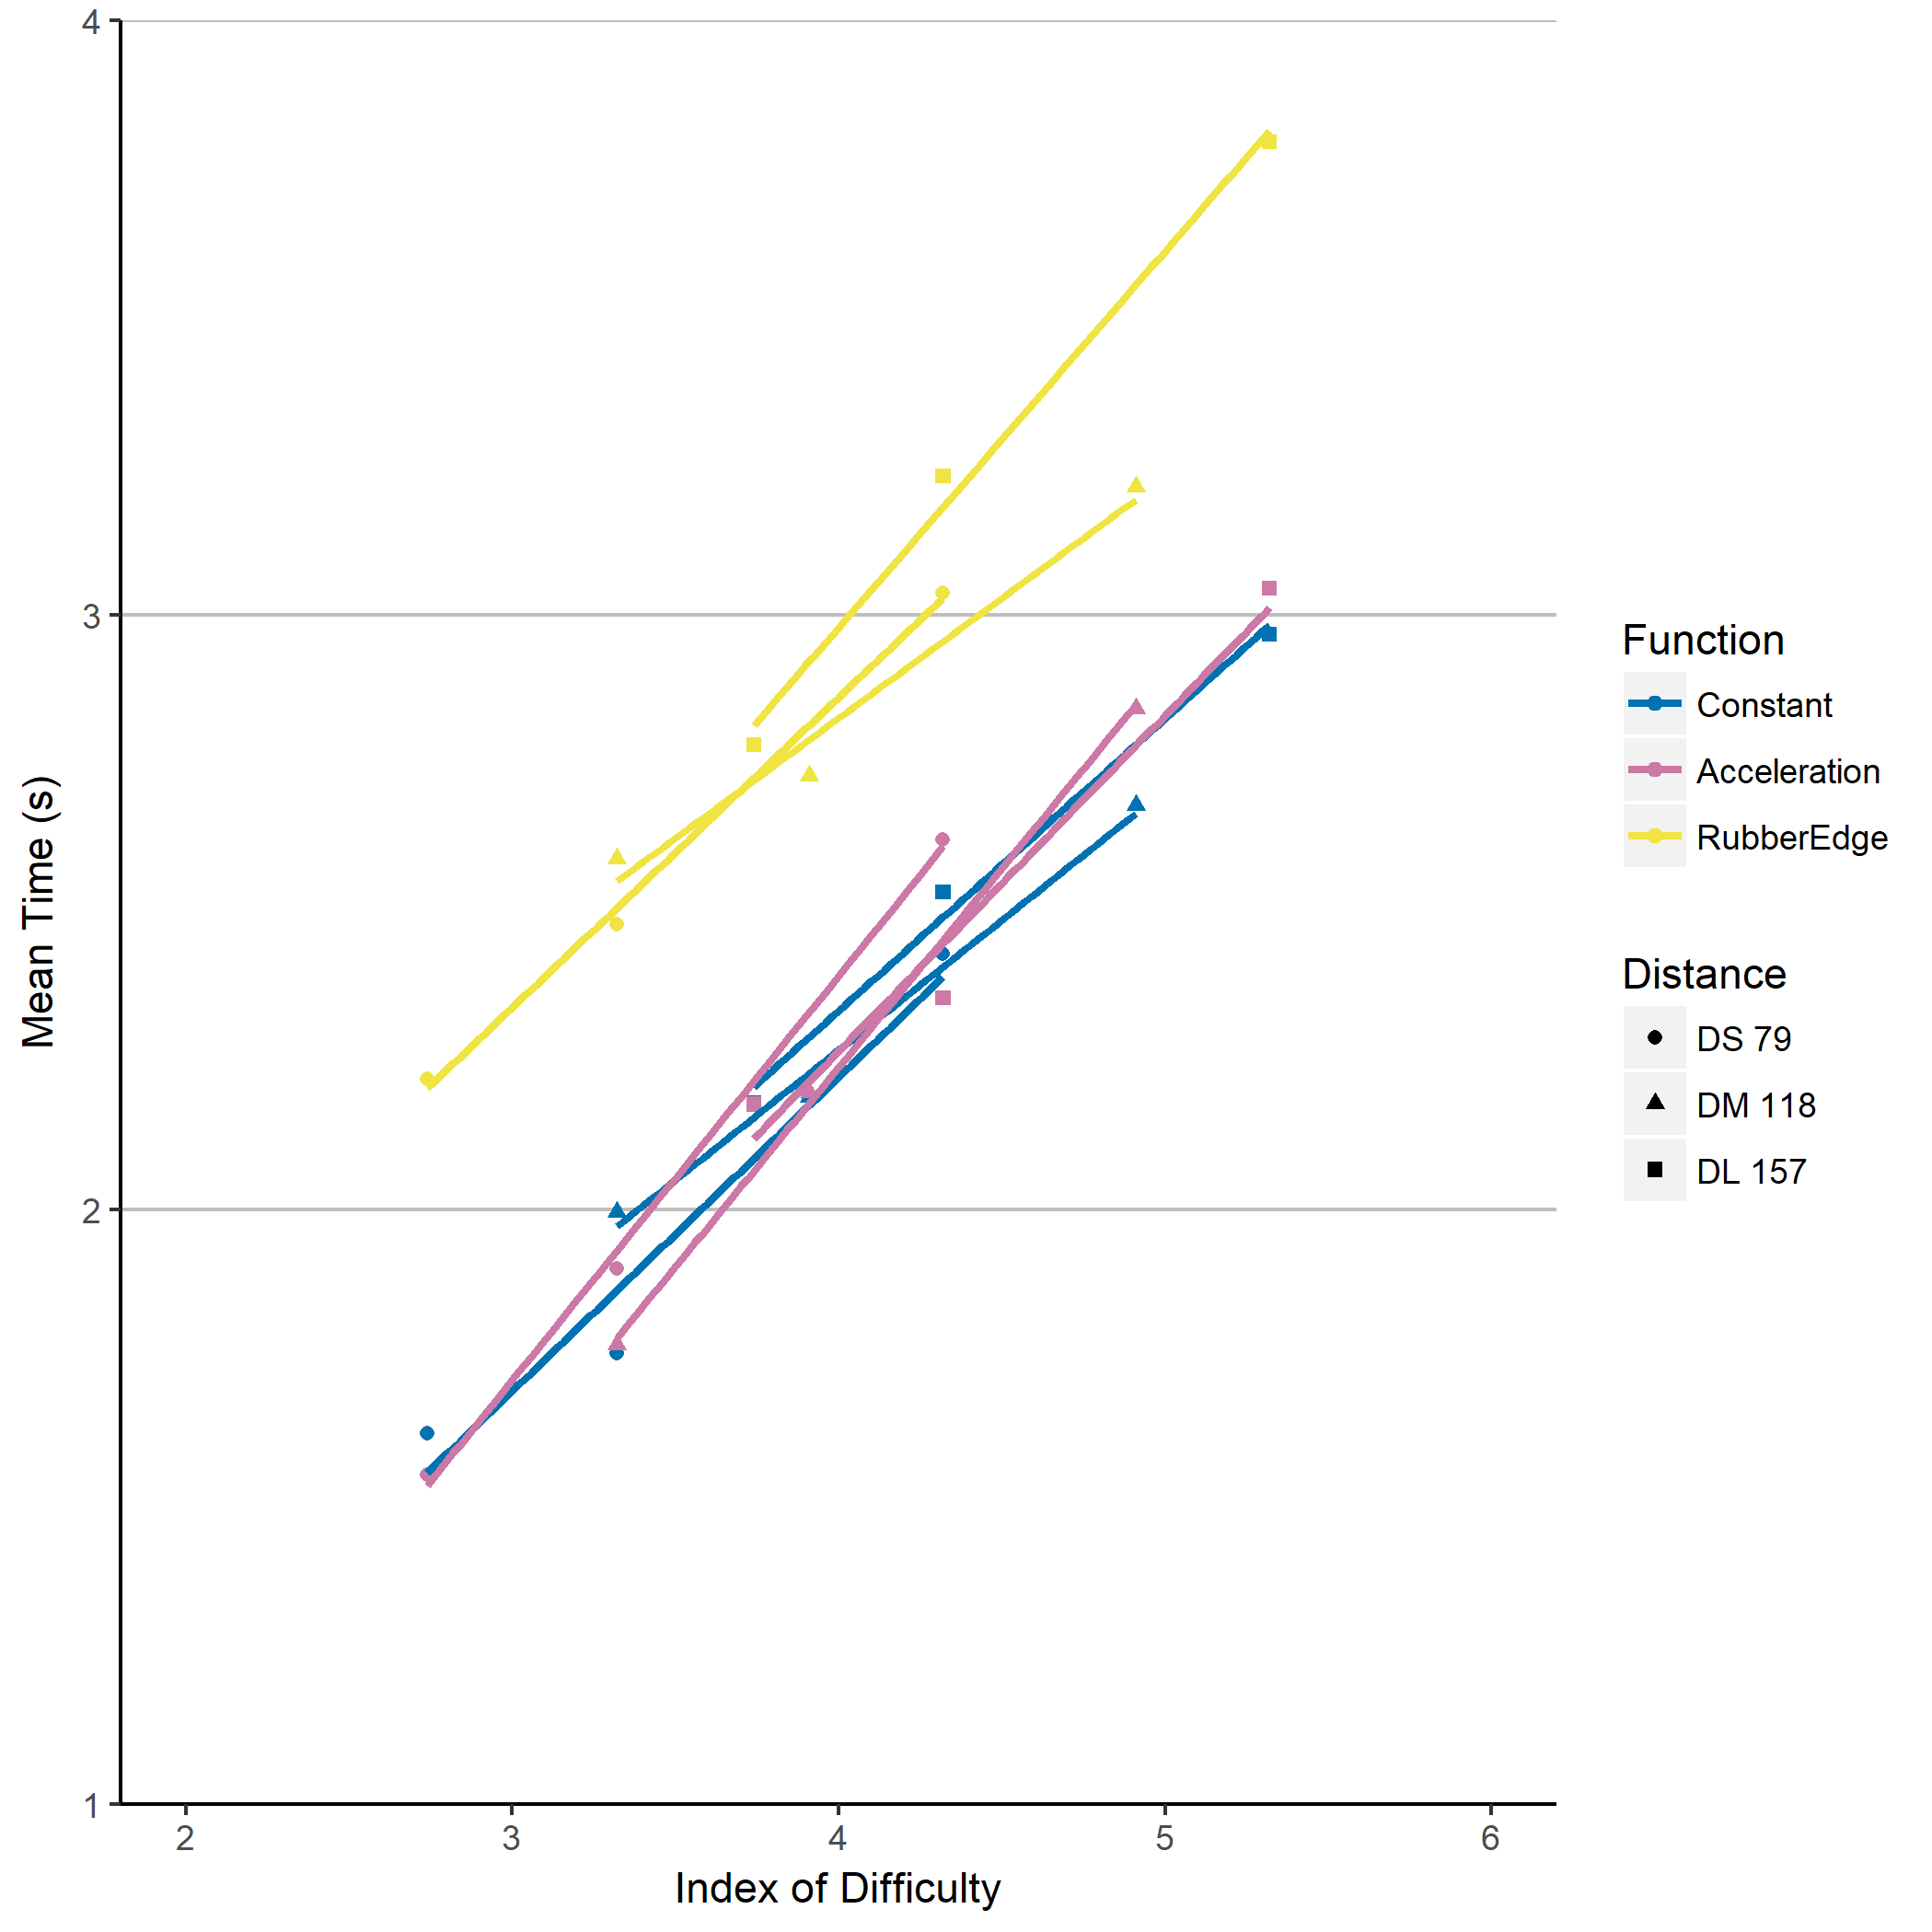
\includegraphics[width=0.9\columnwidth]{fitts-grouped}
    \caption{A comparison between the Index of difficulty and mean time, between different transfer functions, where each distance is separated into its own group.}
    \label{fig:fitts-grouped}
\end{figure}


Table \ref{table:fitts} also shows that the $r^2$ values for each Transfer Function are within acceptable values. For interest, a Figure showing the different distances is also supplied (Figure \ref{fig:fitts-grouped}). This shows that for each Transfer Function the distances are neatly grouped together.

\subsection{Clutches}
Clutches are the number of times a participant removes their finger from the touchpad to continue the task of moving the pointer to a target. This is recorded on a per trial basis.

\begin{figure}[h]
    \centering
    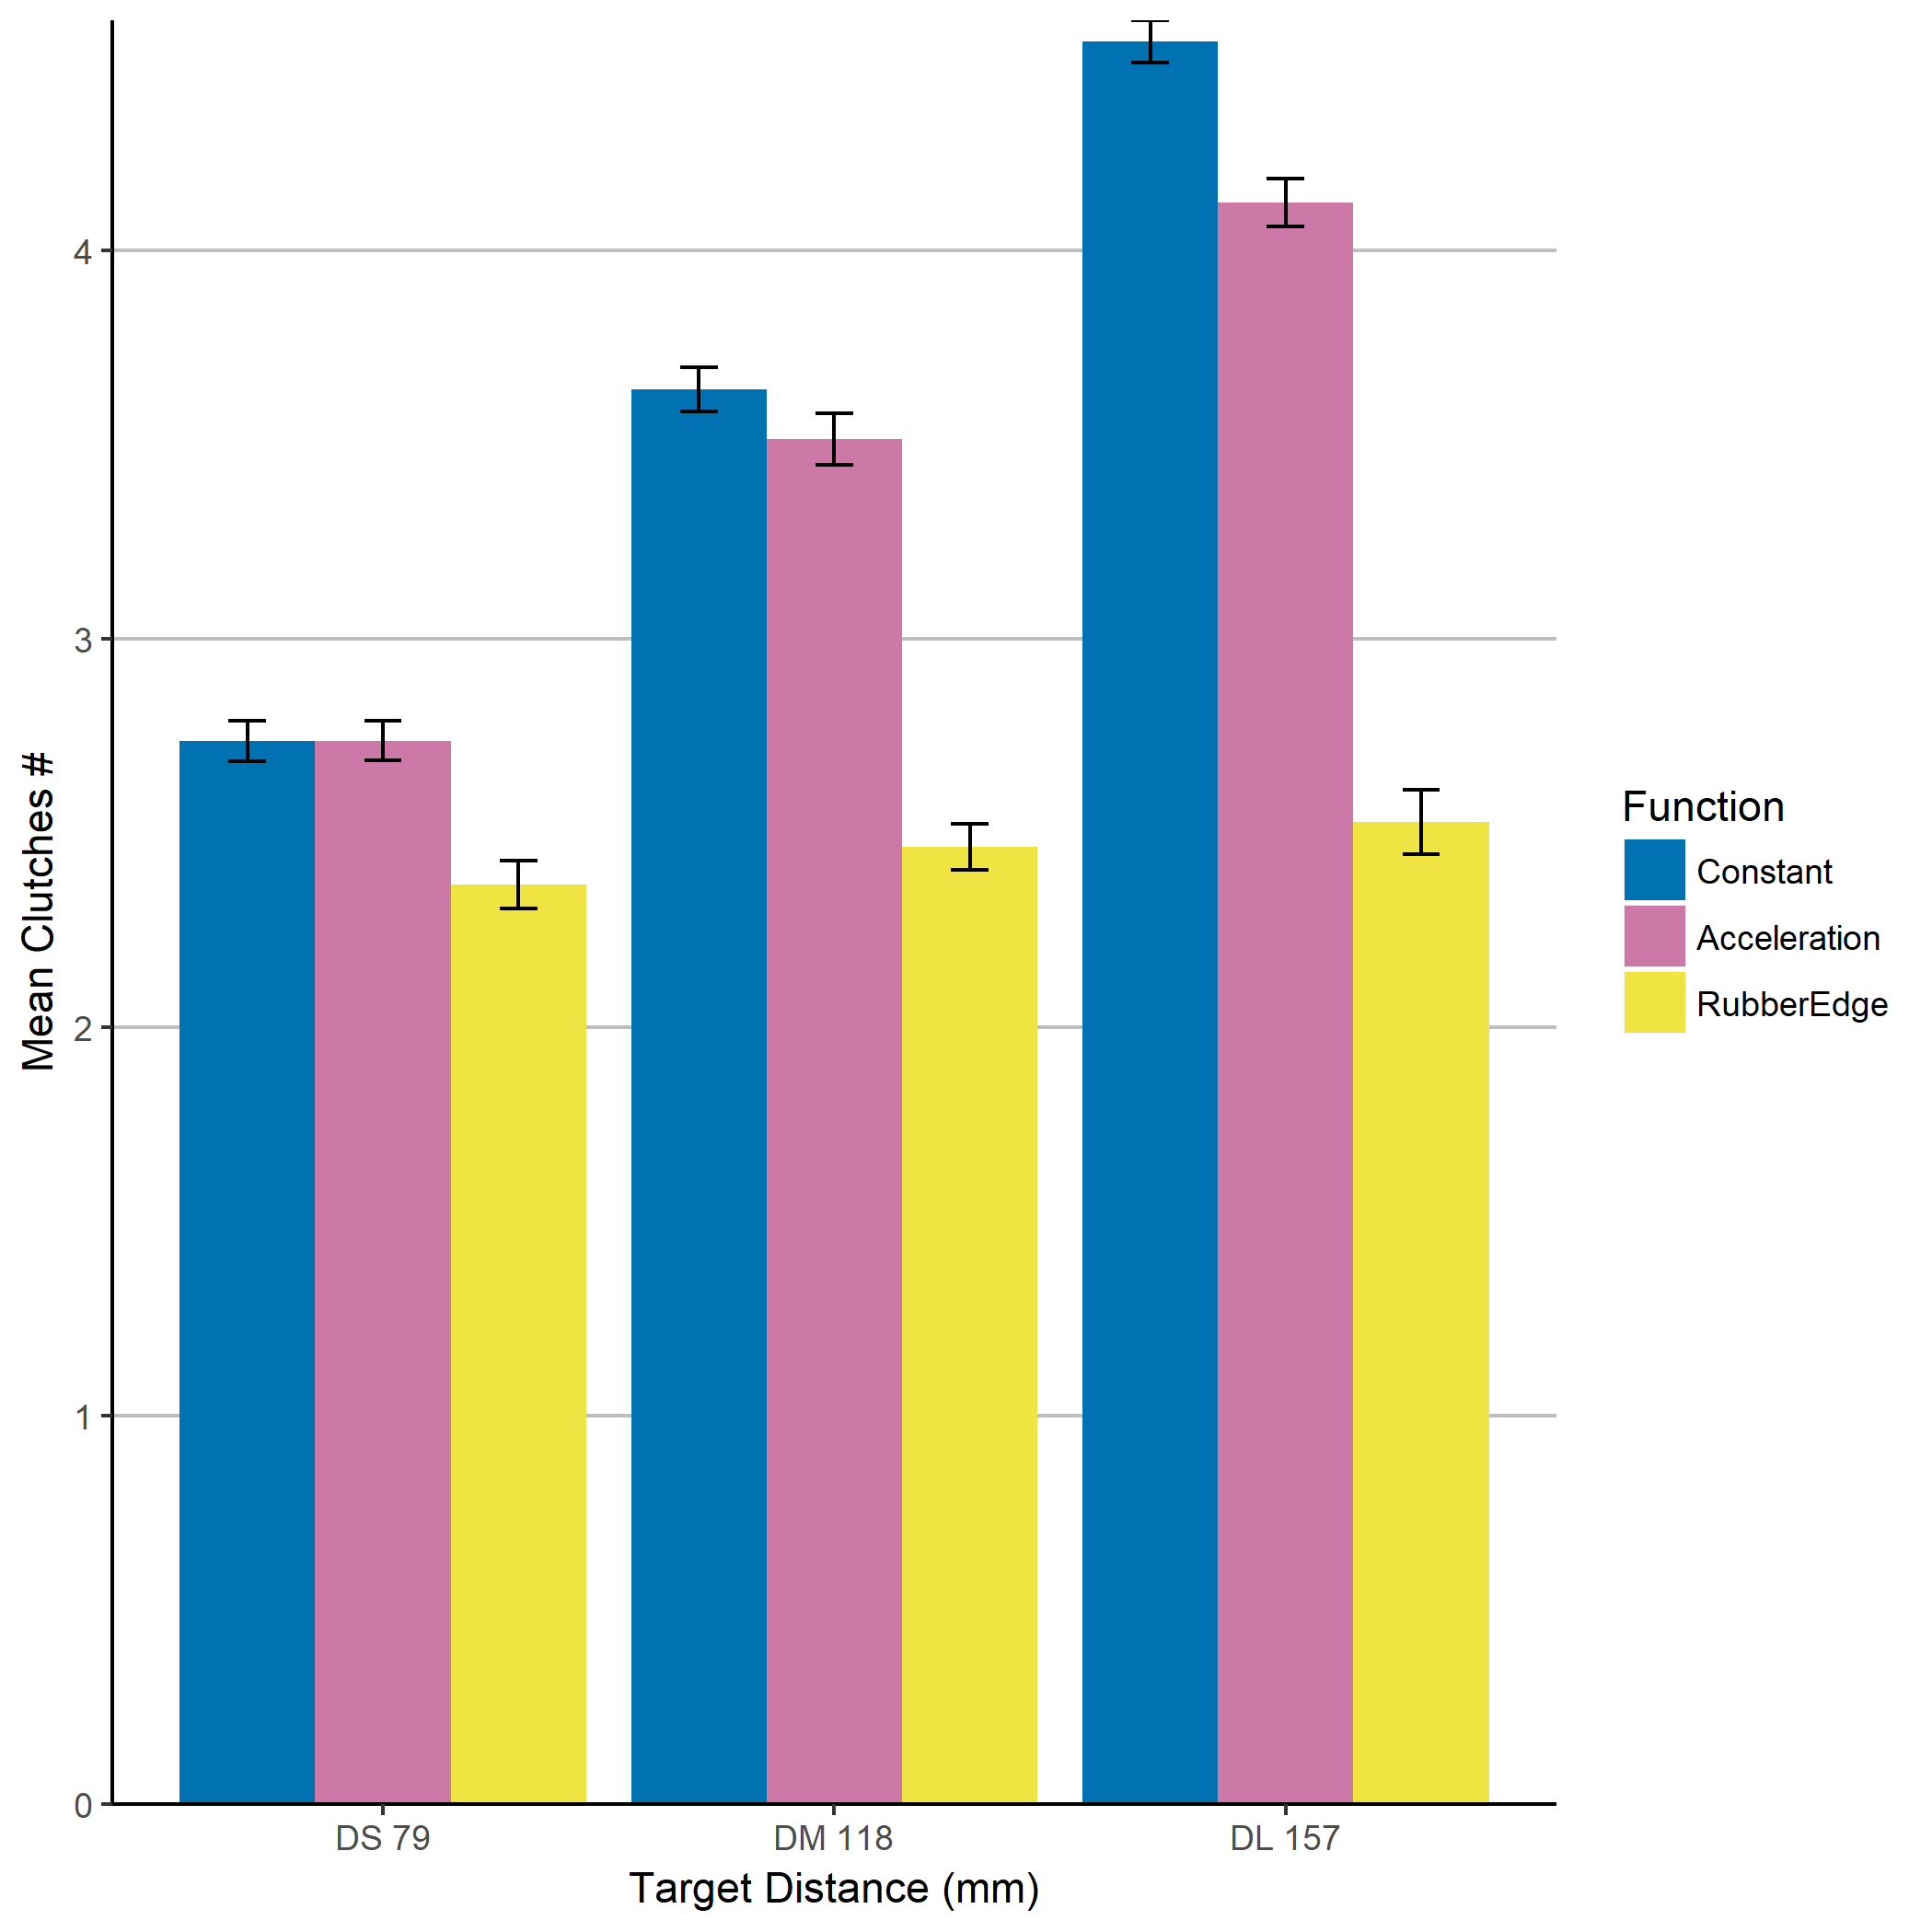
\includegraphics[width=0.9\columnwidth]{clutches}
    \caption{Transfer Function x Distance Interaction on clutch invocations.}
    \label{fig:clutches}
\end{figure}

The order of the Transfer Functions presented to the participants had no significant effect on clutch invocations as found using Mauchly's Test for Sphericity. There was a significant main effect for the Transfer Function on clutch invocations (F$_{2,12}$ = 23.4, p < 0.0001) with the RubberEdge Function outperforming the Constant and Acceleration Function at all Distances. A significant main effect was also present for Distance on clutch invocations (F$_{2,12}$ = 114.2, p < 0.0001). More importantly, there was a significant Transfer Function x Distance interaction (F$_{2,24}$ = 32.2, p < 0.0001), as shown in Figure \ref{fig:clutches}. RubberEdge outperforms both the Constant and Acceleration functions at all Distances (D$_S$, D$_M$, D$_L$) by ~(13.6\%, 31.1\%, 41.6\%) respectively. A pair-wise comparison confirms this finding with both Acceleration vs RubberEdge and Constant vs RubberEdge having p < 0.0001. We therefore accept \textbf{H1}.


\subsection{Participant Feedback}
Participants were asked the following question for each Transfer Function at the end of the experiment. 'Was the interface frustrating to use?', 'Was the interface easy to use?' and 'The interface felt accurate?'. Only the question about accuracy was found to be significant ($x^2_r = 6.42$, df = 2, $p = < 0.05$). Where 5 out of 7 participants agreed that the Constant Transfer Function was accurate, 4 out of 7 agreed that Acceleration was accurate and 4 out of 7 participants found that RubberEdge not to be accurate.

Participants commented the noticeable lag in the pointer see section \ref{section:interface_problems}, which details the issue. 

    \section{Discussion}
Our experiment confirmed the first hypotheses \textbf{H1}, but failed to confirm \textbf{H2}

\subsection{Selection Time}
\textbf{H2} could not be confirmed: RubberEdge Transfer Function would reduce the time taken to traverse a pointer to a target, as there was no significant interaction found between Distance and Transfer Function for selection time. A Log transformation was tried on the data to reduce noise, but this did not make the results significant. This is likely caused by the lag induced by the interface. For the elastic zone, the transfer function used was a naive approach, when compared to the physics-based approach detailed in the source paper\cite{Casiez2007RubberEdge}. Some participants also commented on the fact that the pointer would accelerate to a peak velocity that felt as though they were not in control. This is in spite of the peak limitation of the maximum velocity and suggests that an investigation into the maximum velocity in the elastic zone is needed.

\subsection{Clutches}
Our results confirmed \textbf{H1}: Clutch invocations for the RubberEdge Transfer Function would be less than Constant and Acceleration. When using the RubberEdge function participants would often use a technique where they would enter the elastic zone and slightly overshoot the target, and then proceed to use the isotonic zone to perform the remaining traversal to the target.

\subsection{Apparatus}
One of the key issues with the physical apparatus is the limiting of the usable space for the touchpad; this is not so much of an issue for pointing tasks as 'users tend to focus input in the centre of the touchpad.'\cite{Avera2016EffectsPerformance}. It was also found that 'increased touchpad size did not have a significant effect on the input area that people used for pointing or gestural input.' Although there is evidence that the reduced usable size will not significantly impact a user, the size of the isotonic zone does mean that four finger gestures cannot be used. A better solution for RubberEdge would have the elastic zone built into the touchpad. To induce the feeling of resistance a different texture\cite{SureshBabu2011EffectsAssessments.} could be used, or haptic feedback which emulates a sensation of moving your finger up a slope. However, this type of targeted haptics does not currently exist.

    \section{Conclusion}
RubberEdge enables users to reduce the clutches required to reach pointer targets but maintains the benefits of position control for precise movements. The results show that RubberEdge decreases the number of clutches (14\% - 42\%) for pointer targets at short and long distances. However, the implementation of RubberEdge had a negative effect on selection time; this was primarily due to an inadequate elastic function and lag in the interface. Future iterations of RubberEdge hold promise if the selection time issue can be addressed.

    \section{Future Work}\label{futureWork}
If the experiment was to be repeated, consider using a Macbook Pro touchpad, where access to the \gls{API} for absolute finger position on the touchpad might be easier. This would avoid the use of having to use an iPhone as a touch interface and would eliminate the lag with the existing solution; if this was not possible then consider communicating with the phone over USB. Changing the transition function of the elastic zone for RubberEdge to more closely match the function described in the source paper\cite{Casiez2007RubberEdge}, might help to obtain results that decrease the negative effect on selection time. The study was also limited in the number of participants, increasing this would likely help obtain significant results for selection time.
    
    \balance{}

    \printglossary[type=\acronymtype,title=ACRONYMS]
 
\printglossary

    %*******************************************************
% Bibliography
%*******************************************************
\bibliographystyle{SIGCHI-Reference-Format}
\bibliography{mendeley}

    
    \section{Acknowledgements}
I would like to acknowledge David Read, for help with the printing and cutting of the RubberEdge interface.
Andy Cockburn for putting up with me :)
    
    \section{Appendix}
Github link for source code of project \url{https://github.com/Awarua-/RubberEdge2}


\end{document}
